\documentclass[12pt]{article}
\usepackage[brazil]{babel}
\usepackage[utf8]{inputenc}
\usepackage{graphicx}

\title{Análise de características autonômicas do Google App Engine}
\author{
        Herberth Amaral \\
                Departamento de Ciência da Computação\\
                Programa de Pós Graduação em Modelagem Computacional e Sistemas\\
        UNIMONTES\\
}
\date{\today}

\begin{document}
\maketitle

\begin{abstract}
    O crescente aumento da complexidade de aplicações Web tem levado empresas a
    especializarem seus serviços e delegarem tarefas de infra-estrutura a
    outras empresas especializadas. A comum prática de configurar todo um
    ambiente de implantação de uma aplicação está sendo deixada de lado em
    favor de uma abordagem mais prática e autonômica.  Auto-cura,
    auto-otimização, auto-proteção e auto-configuração, todos elementos da
    computação autonômica, são necessários (e até exigidos) em ambientes PaaS
    (\textit{plataform as a service}), como é o caso do Google App Engine (GAE).
    Este artigo visa analisar cada um dos elementos da computação autonômica do
    GAE e mostra que ele atende satisfatoriamente todos os requisitos.
\end{abstract}

\section{Introdução}
Computação autonômica tem o objetivo de desenvolver de sistemas computacionais
capazes de auto-gerenciamento e adaptação a mudanças imprevisíveis. Alguns
serviços da World Wide Web operam em ambiente hostil e precisam responder a
mudanças de forma rápida e eficiente.

O GAE faz parte de uma nova geração de serviços conhecidos como Plataformas
Como Serviço, ou da sigla em Inglês Paas, que tem como objetivo tirar o fardo
de configuração de um abiente de implantação de aplicações web de empresas que
desenvolvem esses serviços. Com o GAE não é necessário configurar captura de
logs, auto-escala da aplicação, provisionamento de novos servidores,
armazenagem de dados e proteção contra vulnerabilidades de sistema operacional
ou da pilha de software que servirá a aplicação.

O \textit{tradeoff} imposto pelo GAE é o reduzido número de opções. Por
exemplo, não é possível acesar arquivos diretamente do sistema de arquivos, uma
vez que as instâncias são efêmeras, ou seja, podem ser destruídas a qualquer
momento. A análise detalhada dos \textit{tradeoffs} não estão no escopo deste
trabalho, entretanto.

Este trabalho tem o objetivo de analisar os componentes de computação
autonômica do GAE e está dividido nas seguintes seções: a seção 2 trata dos
detalhes do funcionamento do GAE, a seção 3 analisa as capacidades de
auto-cura, a seção 4 analisa as capacidades de auto-otimização, a seção 5
analisa as questões referentes à auto-proteção, a seção 6 analisa as
características de auto-configuração e a seção 7 delineia as considerações
finais.

\section{Detalhes de funcionamento do GAE}

Esta seção mostra a mecânica envolvida no gerenciamento de aplicações/projetos
do GAE. No geral, não há quesitos desafiadores, uma vez que os detalhes mais
complicados são gerenciados pelo próprio GAE.

\subsection{Interface com o usuário}
Com o intuito de diminuir a fricção nas configurações do ambiente da aplicação,
o GAE possui uma rica interface capaz de configurar aspectos básicos e
avançados do ambiente da aplicação. É importante notar que tais configurações
não impactam no requisito de auto-configuração dos sistemas autonômicos, pois
essas são feitas apenas uma vez. 

A figura \ref{fig:painel} mostra a interface de usuário inicial do GAE.
\begin{figure}
    \centering
    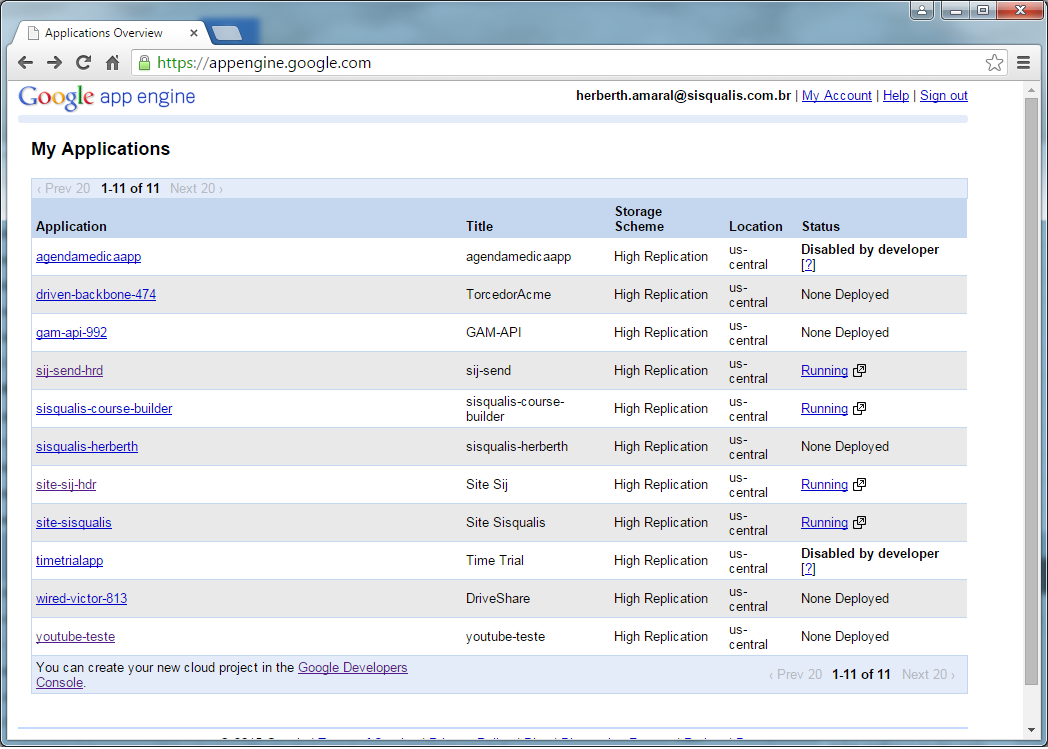
\includegraphics[width=0.75\textwidth]{painel.png}
    \caption{Página inicial do GAE (fonte própria)}
    \label{fig:painel}
\end{figure}

A figura \ref{fig:novoprojeto} mostra as configurações necessárias para criar
um projeto: apenas o nome e localização geográfica. Para uma aplicação padrão
do GAE, estas são as únicas configurações necessárias.

\begin{figure}
    \centering
    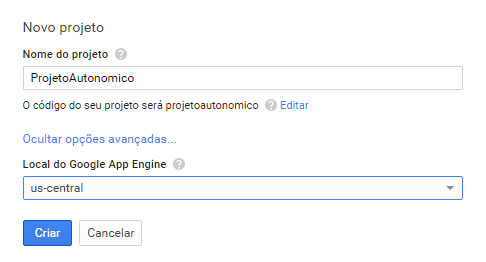
\includegraphics[width=0.75\textwidth]{novoprojeto.png}
    \caption{Interface de criação de um novo projeto no GAE (fonte própria)}
    \label{fig:novoprojeto}
\end{figure}

O painel específico de cada aplicação provê estatísticas em tempo real de
acesso, erros e outros dados de execução do projeto. A figura
\ref{fig:painel-app} mostra um exemplo do painel da aplicação. Ainda é possível
customizar o que é exibido no painel.

\begin{figure}
    \centering
    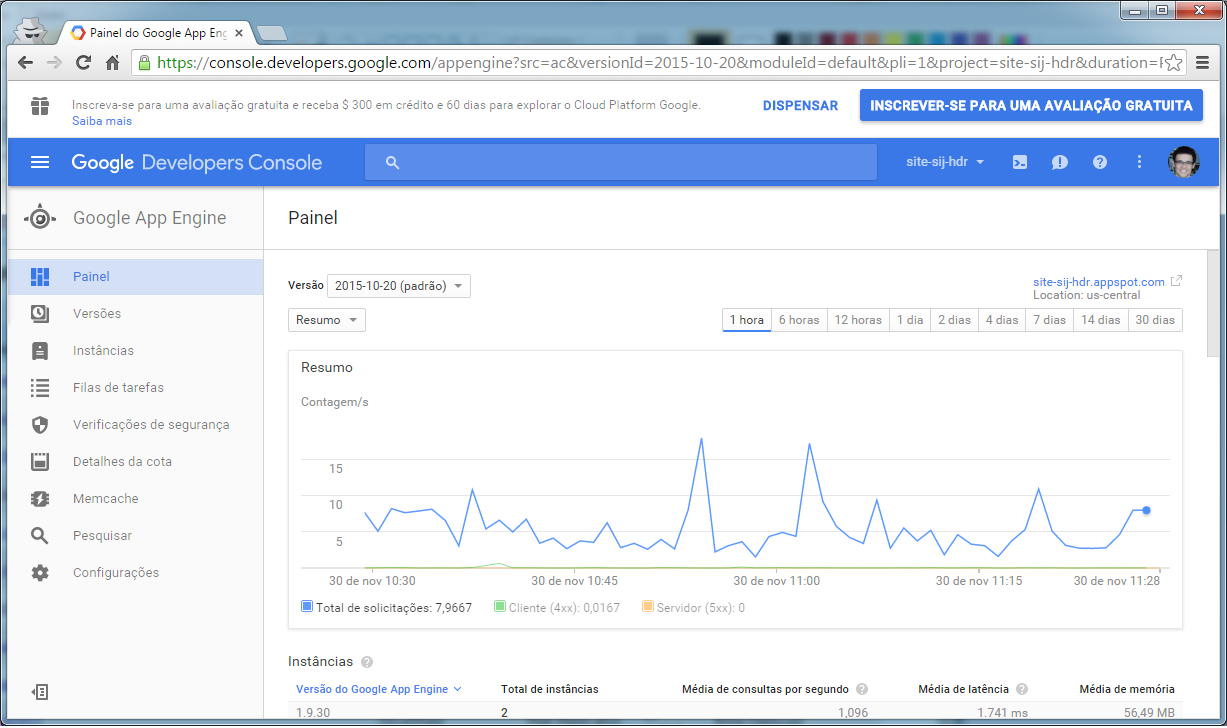
\includegraphics[width=0.75\textwidth]{painel-app.png}
    \caption{Painel específico de uma aplicação (fonte própria)}
    \label{fig:painel-app}
\end{figure}

Dependendo da carga de serviço da aplicação, o GAE provisiona novas instâncias
capazes de aumentar a capacidade de processamento das requisições extras. A
figura \ref{fig:instancias} mostra a lista de instâncias de uma aplicação em um
determinado instante.

\begin{figure}
    \centering
    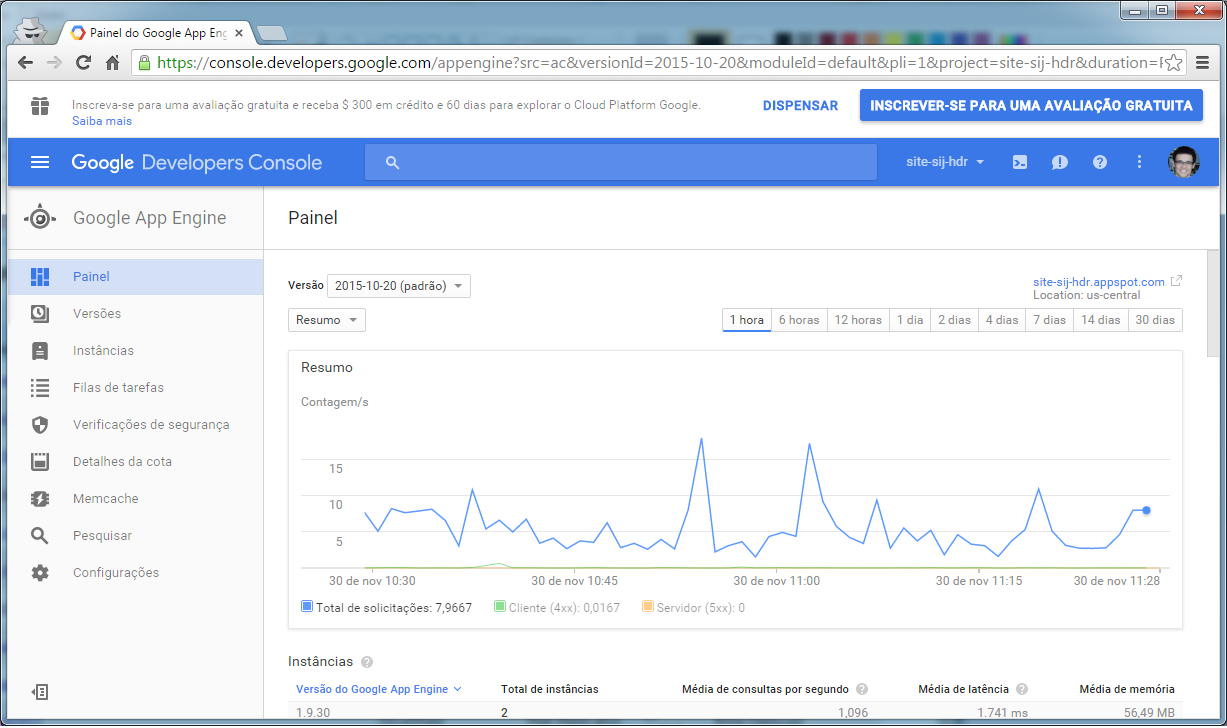
\includegraphics[width=0.75\textwidth]{painel-app.png}
    \caption{Instâncias da aplicação (fonte própria)}
    \label{fig:instancias}
\end{figure}

\subsection{Serviços disponíveis}
\subsection{Configuração dos elementos autonômicos}
\section{Auto-cura}
\section{Auto-otimização}
\section{Auto-proteção}
\section{Auto-configuração}
\section{Considerações finais}

\end{document}
This is never printed
